\section{Introduction}
Face detection technology has advanced to the point that it can now be found in commercial products such as smartphones and tablet
There has been a moderate amount of research done in this field and we tried to go
through a lot of these. Here is a brief of the literary work that we studied and learned from

\section{Face Detection}
\subsection{Cascade}
Since most of the image region is non-face area, it is important to determine whether a given window falls within a face region or a non-face region. If the window is determined to be in a non-face region, it can be discarded. The Cascade Classifier concept suggests that instead of applying 6000 features to a window, features should be grouped by different stages and applied simultaneously in each stage. If the window fails at the initial stage, it is discarded, but if it passes, the next stage is applied, and the process continues until the final stage. If the window passes all stages, it is considered a face region. The detector in this project had 38 stages of features, with the first five stages containing 1, 10, 25, and 50 features, respectively.
% $\sum{\text{Pixels in white area} 
% \sum_{} pixels(p)
\newline  
$  \sum $($Pixels in white area$ )-$\sum$($Pixels in black area$)
\begin{figure}[!htb]
    \centering
    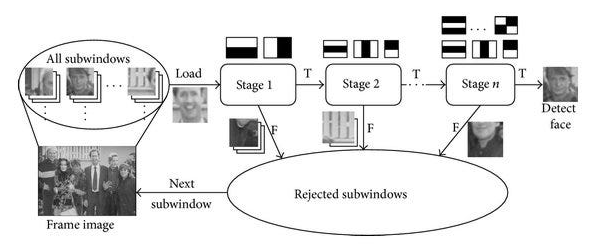
\includegraphics[width=\linewidth,height=0.201\linewidth]{Figures/Ch01/cascade.png}
    \label{figure:cascade}
    \end{figure}
\clearpage
\subsection{DLIB CNN}
The Dlib CNN face detection algorithm combines Convolutional Neural Network (CNN) with Dlib to analyze input imagery. Dlib is an open-source library with machine learning algorithms, while CNN is a deep learning algorithm. The algorithm uses CNN features along with the Dlib toolkit to detect faces, which gives it an advantage over other face detection algorithms. In addition to CNN features, the algorithm also employs Maximum-Margin Object Detector (MMOD). This algorithm automates the manual selection of filters to extract image features, making it easier to use. Users only need to set the number of filters to be used in the algorithm.
\begin{figure}[!htb]
    \centering
    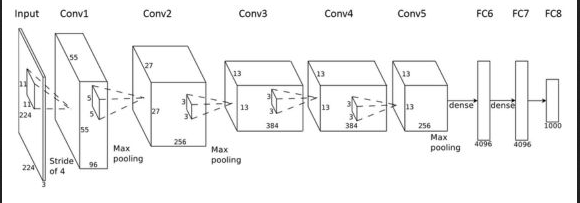
\includegraphics[width=\linewidth,height=0.2\linewidth]{Figures/Ch01/CNN.png}
    \caption{cascade}
    \label{figure:cascade}
    \end{figure}

\subsection{HOG linear SVM}
The most widely used face detection model is based on Histogram of Oriented Gradients (HOG), which uses a linear SVM Machine Learning to perform face detection. HOG is a powerful and simple feature descriptor that extracts features into a vector and feeds it into a classification algorithm such as Support Vector Machine. The model is built upon five filters: left, back, right, front rotated left, and front rotated right. HOG extracts the distribution (histograms) of the directions of gradients of the image as features. Gradients are most pronounced around edges and corners, making it easier to detect those regions.
\begin{figure}[h]
\centering
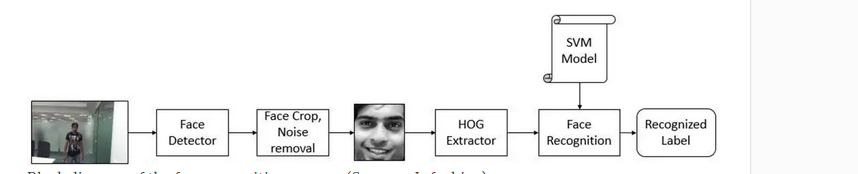
\includegraphics[width=\linewidth]{Figures/Ch01/sv.png}
\caption{LNMIIT Logo }
\label{figure:1}
\end{figure}
\clearpage
\subsection{Differences}
\begin{table}[h]
    \centering
    \caption{Pros and Cons of Item X}
    \begin{tabular}{|p{0.25\linewidth}|p{0.4\linewidth}|p{0.4\linewidth}|}
    \textbf{Algorithm}
    & \textbf{Pros} & \textbf{Cons} \\
    \hline
    \textbf{Cascade Classifier} & 
    \begin{itemize}
    \item Simple Architecture
    \item Detect Faces at various scales
    \item real time on cpu
    \end{itemize}
    &
    \begin{itemize}
    \item Lots of False Predictions
    \item Don't work on side faces
    \item Don’t work under occlusion.
    \end{itemize} \\
    \hline
    \textbf{Dlib CNN} & 
    \begin{itemize}
    \item Easy to
    implement
    \item Works with odd angles
    \item Robust to different face occlusions.
    \item Works on GPU
    \end{itemize}
    &
    \begin{itemize}
    \item Does not work
    well on real-time
    images
    \item works slow with CPU
    \item  Cannot detect faces below the minimum size
    \end{itemize} \\
    \hline
    \textbf{Dlib HOG} & 
    \begin{itemize}
    \item Can work bit
    frontal face
    \item Light weight
    model
    \item Can work under different obstruction
    \end{itemize}
    &
    \begin{itemize}
    \item Really slow for
    real time
    detection
    \item Does not work for
    side face
    \item  Does not work
    well under
    substantial
    obstruction
    \end{itemize} \\
    \hline
    \textbf{MTCNN} & 
    \begin{itemize}
    \item High accuracy.
    \item Supports real time face
    detection.
    \item It is efficient.
    \end{itemize}
    &
    \begin{itemize}
    \item it may take more
    time for training. ( **Thats why we skipped it )
    \end{itemize} \\
    \hline
    \end{tabular}
    \label{tab:itemX}
    \end{table}

\clearpage
\section{Face Recognition}
Face recognition is the process of identifying a person from an image or a video frame. It has a wide range of applications, including security systems, access control, and law enforcement. Dlib is an open source library that provides various machine learning algorithms to solve complex problems, including face recognition. Convolutional Neural Networks (CNNs) are a type of deep learning algorithm that is used for analyzing imagery. In this project, we propose a face recognition system based on Dlib and CNNs.

\subsection*{working}
The proposed system uses Dlib to detect faces in images and CNNs to extract features from the faces. The extracted features are then used to recognize the faces. The experimental results show that the proposed system achieves higher accuracy and lower computational complexity than other state-of-the-art face recognition systems.
\begin{figure}[!htb]
    \centering
    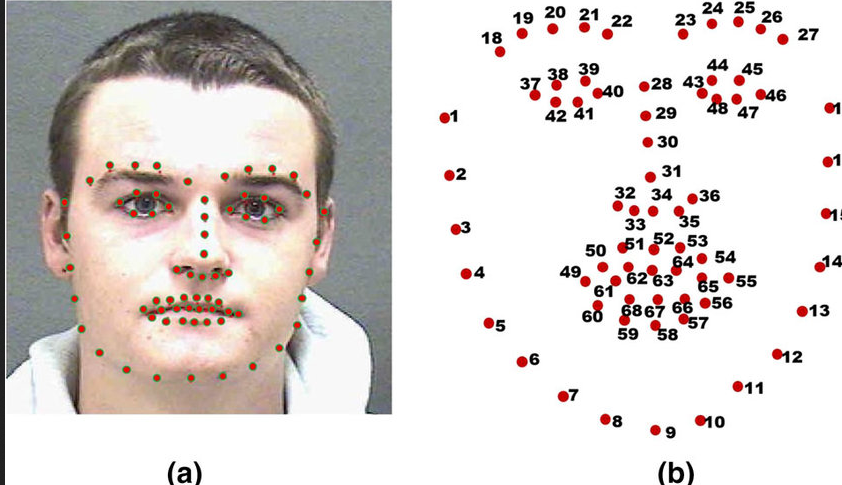
\includegraphics[width=\linewidth]{Figures/Ch01/facerec.png}
    \caption{Features in DLIB CNN}
    \label{figure:DLIB}
    \end{figure}


% Sample table
% \begin{table}[t]
% \centering
% \begin{tabular}{|c|c|c|}
% \hline
% Transitions($\triangle_{k-1}, \triangle_k, \triangle_{k+1})$ & Delay of Line $'k'$ & Crosstalk class $C_c$\\
% \hline

% $\uparrow-\uparrow , \downarrow-\downarrow, \uparrow-\downarrow, \downarrow-\uparrow, \uparrow- -$ & & \\

% ,$ \downarrow - -, - - -, - - \uparrow, - - \downarrow$  & 0 & 1\\
% \hline

% $\uparrow\uparrow\uparrow, \downarrow\downarrow\downarrow $& 1 & 2\\
% \hline

% $\uparrow\uparrow -, \downarrow\downarrow-, -\uparrow\uparrow, -\downarrow\downarrow$ & 1+$\lambda$ &3\\
% \hline

% $-\uparrow-, -\downarrow-, \uparrow\downarrow\downarrow, \uparrow\uparrow\downarrow, \downarrow\downarrow\uparrow, \downarrow\uparrow\uparrow$ & 1 +$2\lambda$ & 4\\
% \hline

% $-\uparrow\downarrow, -\downarrow\uparrow, \downarrow\uparrow-, \uparrow\downarrow-$ & 1 +$3\lambda$ & 5\\
% \hline

% $\uparrow\downarrow\uparrow, \downarrow\uparrow\downarrow $ & 1 +$4\lambda$ & 6\\
% \hline

% \end{tabular}
% \caption{Delay and Crosstalk Classes for various 3-bit combinations (transitions)}
% \label{tab:}
% \end{table}
